%------------------------------------------------------------------------------------------------------------
\section{Database management} \label{sec:DataBases}
%------------------------------------------------------------------------------------------------------------

This section covers the description of databases that will be used by AMIDST learning and inference algorithms implemented in the toolbox.  Figure~\ref{fig:DataBase} shows a high-level overview of the key components of the AMIDST software tool. It illustrates mainly the different database functionalities and how they are connected to the core component \comp{PGM} through both the \comp{Learning Engine} and \comp{Inference Engine} components. In what follows, we describe each of the database functionalities, along with a code excerpt containing a brief example how to define the described functionality., then introduce briefly the \comp{Learning Engine} and \comp{Inference Engine} that will be presented in more details in Deliverable 3.2.

  \begin{figure}[htbp]
    \centering
    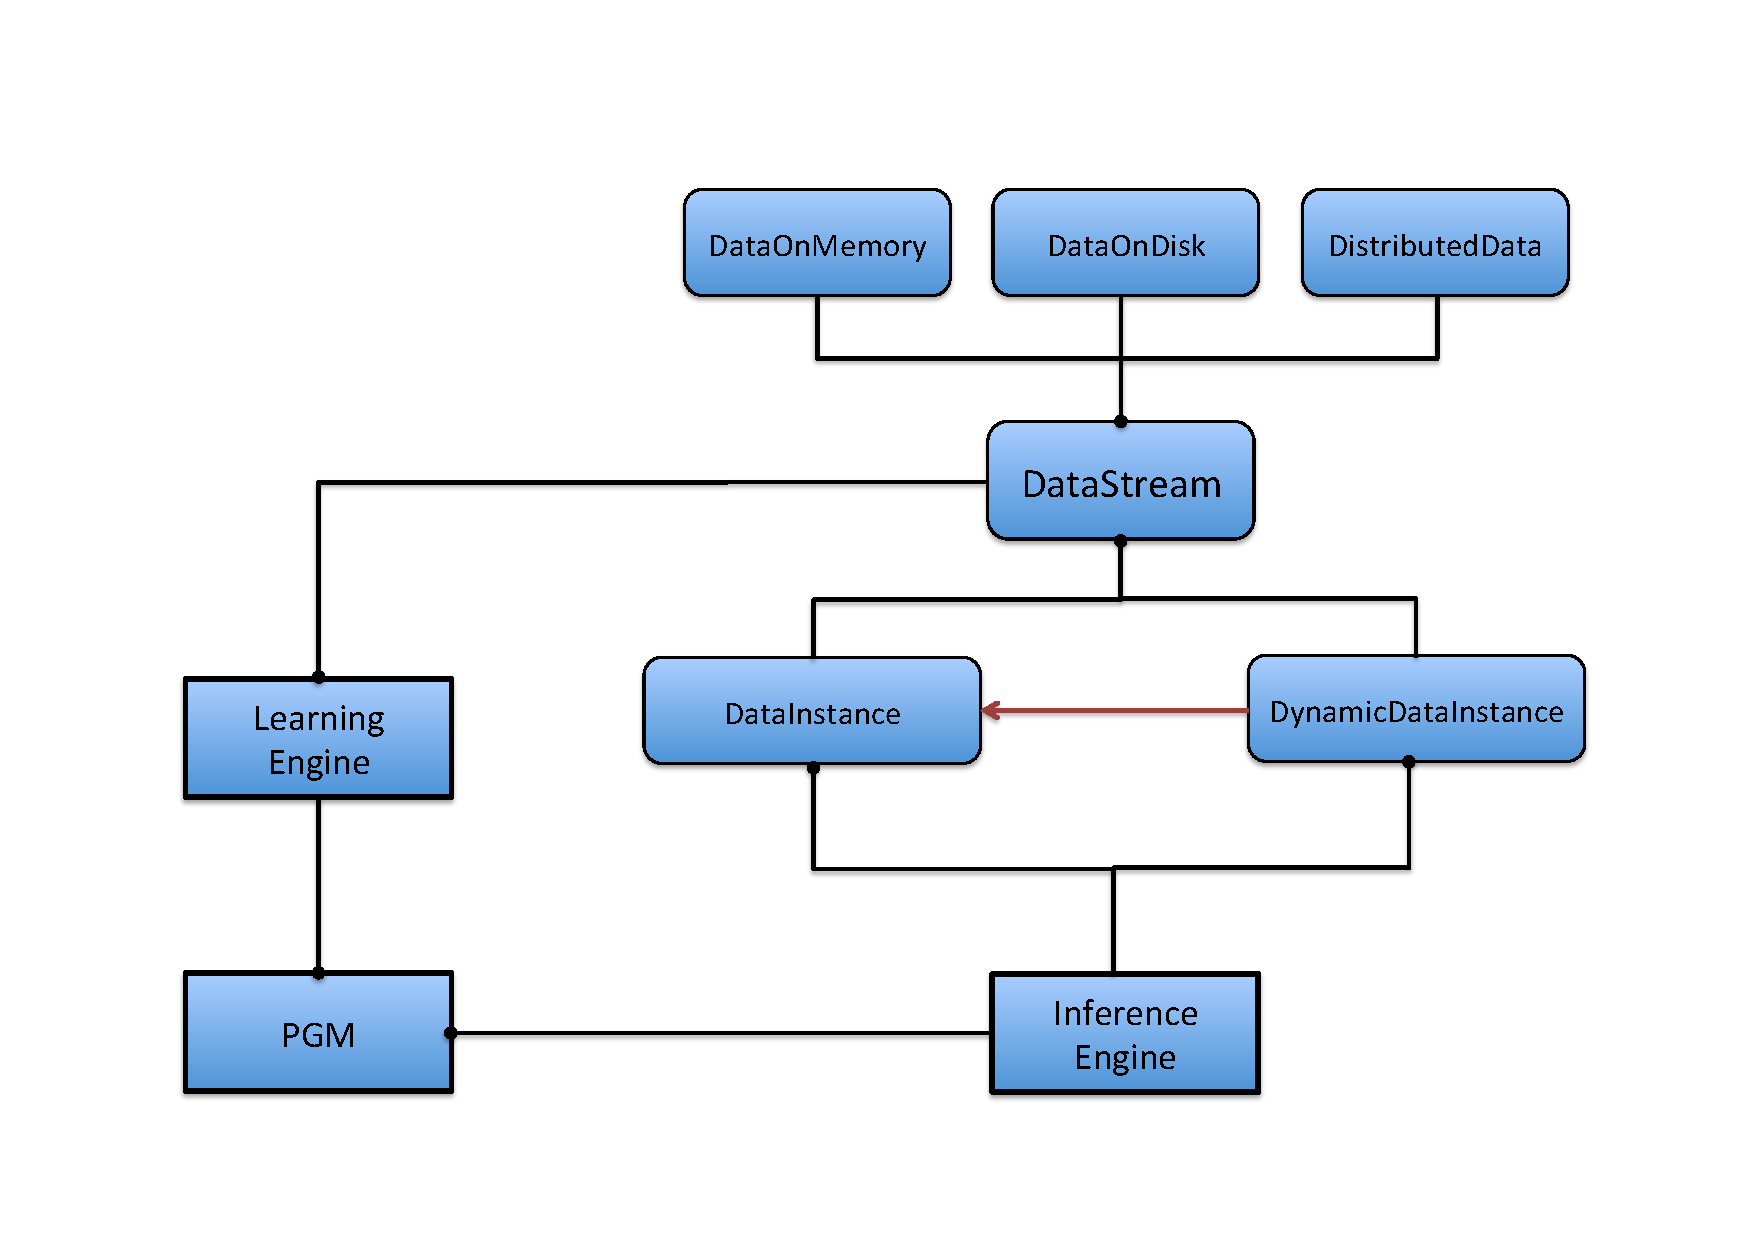
\includegraphics[width=1.05\linewidth]{./figures/DataBase}
    \caption{Illustration of the main database management functionalities and their connection with PGM, learning engine, and inference engine components. }
    \label{fig:DataBase}
  \end{figure}
 
%------------------------------------------------------------------------------------------------------------
\subsection{DataStream}
%------------------------------------------------------------------------------------------------------------   

In the AMIDST framework, we consider a streaming data as a data source, where data arrives at high frequency with no storage of historical data. Then, from this general (\comp{Data Stream}) component, the specialised database functionalities could be derived, namely, (\comp{DataOnMemory} and \comp{DataOnDisk}.

In addition, Data Stream is connected to \comp{Data Instance} and \comp{Dynamic Data Instance} components. 

The employed design is intended to support future users and developers of the AMIDST toolbox in the potential design and implementation of other database specifications; the only restriction being that new database components should implement the interface defined by the \comp{Data Stream} component. 

%------------------------------------------------------------------------------------------------------------
\subsection{DataOnMemory}
%------------------------------------------------------------------------------------------------------------  

\comp{DataOnMemory} implements database functionality for data sets that can be loaded into main memory.

%------------------------------------------------------------------------------------------------------------
\subsection{DataOnDisk}
%------------------------------------------------------------------------------------------------------------  

\comp{DataOnDisk} provides functionality for handling datasets too large to be loaded in main memory.

%------------------------------------------------------------------------------------------------------------
\subsection{DataInstance}
%------------------------------------------------------------------------------------------------------------  
  
The \comp{Data Instance} component consists of a single class that can represent a particular evidence configuration, such as the observed values of a collection of variables at time $t$ or a particular row in a database. 

%DataInstance refers to a row in the data set typically containing a value assignment for each attribute. In terms of code, DataInstance is defined as an interface that is implemented by either a StaticDataInstance or a DynamicDataInstance. The former stores one row (DataRow) of the data set at a time, whereas the second stores two rows of the data set (one for the past and another for the present). 
  
%------------------------------------------------------------------------------------------------------------
\subsection{DynamicDataInstance}
%------------------------------------------------------------------------------------------------------------  

The \comp{DynamicDataInstance} always has a TimeID and a SequenceID. If this two attributes, or any of the two, are not in the dynamic data set, then they are automatically filled in, incrementally for the TimeID and with a value of $1$ for the SequenceID.

%------------------------------------------------------------------------------------------------------------
\subsection{Learning Engine}
%------------------------------------------------------------------------------------------------------------  

Implementations of learning algorithms will be provided through \comp{Learning Engine} component for static and dynamic Bayesian networks, ensuring both the structural and parameter learning.

For structural learning, the AMIDST toolbox design includes components for supporting PC and TAN learning in a parallel setting (cf.\ Task 4.1). The current implementation supports standard PC learning and parallel TAN learning by interfacing to the Hugin API. 

For parameter learning, a fully Bayesian approach is pursued in the AMIDST framework (cf.\ the activities in Task 4.2 and Task 4.4). This, in turn, means that parameter learning reduces to the task of inference for which we plan to consider two approaches: variational message passing and expectation propagation. More implementation details about these two algorithms will be provided in Deliverable 3.2. 
 
Note that the design of the learning engine of the AMIDST framework is flexible in the sense that it easily accommodates potential future learning-based extensions of the framework, e.g., Bayesian learning based on importance sampling or maximum likelihood learning using the expectation maximization algorithm (see Section 3 in Deliverable 4.1 \cite{Deliverable4.1}). 
 
%------------------------------------------------------------------------------------------------------------
\subsection{Inference Engine}
%------------------------------------------------------------------------------------------------------------  

As previously noted in Deliverable 4.1 \cite{Deliverable4.1} (see Section 3), efficient implementations of both variational message passing and expectation propagation algorithms can be realized when the distribution families of the models are conjugate-exponential. In this case, the inference operations can be further supported by specifying the exponential distributions using their natural parameters. 

These functionalities are ensured in AMIDST toolbox through tailored exponential family implementations of the standard distributions that are part of the AMIDST framework (such as the conditional linear Gaussian distribution). 


  